\documentclass[../talk.tex]{subfiles}
\begin{document}


\begin{frame}{Certificates}
    \begin{overlayarea}{\slidewidth}{\slideheight}
        We need algorithms that also compute \alert{certificates}

        \vspace*{1em}

        \begin{center}
            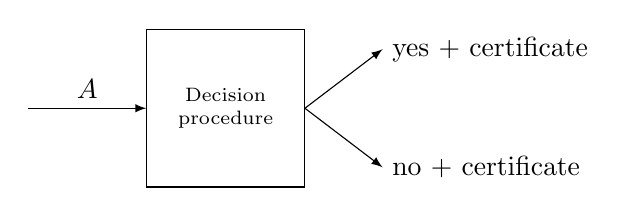
\begin{tikzpicture}
                % \node (origin) [coordinate] at (0.5,0) {};

                \node (rect) at (5,0) [minimum width=2cm,minimum height=2cm, anchor=west,draw] {};

                \node (yes) [coordinate] at (8,0.75) {};
                \node (no) [coordinate] at (8,-0.75) {};
                \path [->,>=latex]
                    (3.5,0) edge (rect.west)
                    (rect.east) edge (yes)
                    (rect.east) edge (no)
                ;

                \node at (4.25,0.25) {$A$};

                \node [right of=yes, node distance=0cm, anchor=west] {yes + certificate};
                \node [right of=no, node distance=0cm, anchor=west] {no + certificate};

                \node [align=center, text width=2cm, font=\scriptsize] at (rect) {Decision procedure};
            \end{tikzpicture}
        \end{center}

        \vspace*{1em}

        \sonslide<2->%
        {%
            A certificate is \alert{additional information justifying} the boolean answer

            \vspace*{1em}
        }

        \sonslide<3->%
        {%
            A certificate can be used to \alert{check} the correctness of the answer

            \vspace*{1em}
        }

        \sonslide<4->%
        {%
            This check should be \alert{easier} than the original computation
        }

    \end{overlayarea}
\end{frame}

\end{document}
